\section{Qualitative Evaluation}

The interaction paradigm of SimpleSpeech was tested in a qualitative assessment to determine (1) the practicability of a lightweight text-based audio editor, (2) the effects of minor transcription errors on audio consumption and production, and (3) the implications of being able to edit audio in an asynchronous online discussion.

Participants were introduced to the functionality of the system, then given two untimed tasks. 
First, to simulate an asynchronous audio discussion, the test users were asked to listen to an audio comment left by the previous tester and create an original audio response. 
Next, they received a different, textual prompt and created an audio comment which would be consumed by the next user. 
In both cases the user was asked to edit his or her recording to be polished and clear.
The participants were interviewed at the end of the test; these interviews were transcribed, conversational elements filtered out, and the remaining sentences analyzed via open coding followed by flat coding. Cohen's $\kappa$ was .78, indicating high reliability between the two coders.

The sample for the study consisted of 9 test subjects (4 male, 5 female, mean age 21.6 yrs; henceforth denoted $P_1, P_2, \ldots, P_9$). 
All participants were native English speakers. 
Two individuals, $P_2$ and $P_3$, were professional media editors who provided technical feedback and a comparison to pure audio editing; the remainder were interns and high school students.

\subsection{Results}
The coding process resulted in the following themes identified from the user feedback:

\emph{The text-based editing paradigm provides sufficient control to render waveform manipulation unnecessary.}
Most non-professional users felt SimpleSpeech gave them ``plenty of control'' over the editing process ($P_4,\,P_5,\,P_6,\,P_8$). 
The professional editors did note that most people in their field would not find SimpleSpeech adequate for their needs; but, as $P_2$ conceded, the intended market users ``don't have to play with the settings which is why they don't use a professional audio editor.''
Most participants characterized the editing experience as being a text-focused one, suggesting that the translation to text was in fact a useful proxy for editing audio. 
The text modality was described as ``more accessible, more doable'' than pure waveform editing, which could be ``scary for people who don't do video stuff'' ($P_3,\,P_7$). 

\emph{The primary use of lightweight voice editing is to make fine-grained rather than large-scale adjustments.}
The most commonly-used manipulation during the qualitative study was the removal of disfluencies ($P_1,\,P_2,\,P_4,\,P_5,\,P_7$), followed by pause deletion ($P_2,\,P_3,\,P_5,\,P_6,\,P_8$). 
Only $P_1$ and $P_8$ edited large chunks of audio by deleting or rerecording, and $P_8$ reported doing so only to improve the smoothness of a smaller change in a sentence.
Perhaps because SimpleSpeech was presented as a tool to be briefly used to ``clean up'' recordings, participants focused on removing the ``embarrassing'' and ``awkward'' sounds ($P_1,\,P_5$).

\emph{Transcription is a helpful aid for listening to audio comments despite occasional errors.}
In many cases, the transcription proved to be an essential element of both the production and the consumption interfaces. 
To determine the effect of errors in the transcript on listeners, the previous participants' comments were displayed to users with an unedited, errorful ASR transcript. 
Despite the occasional errors, users still found the transcript to be helpful in allowing them to ``see all the points [the speaker was] making instead of having to remember them'' ($P_4,\,P_6$). 
For some users, the transcription caused no problems in comprehension, while others experienced errors that required them to pay more attention to the audio ($P_8$). 
On the whole, ASR succeeded in ``getting the basic idea across'' ($P_3$) but could not stand alone without the original recording. 

\emph{The linearity of audio leads to a pressure to organize one's thoughts during recording.}
$P_4,\,P_7,$ and $P_9$ described a ``psychological sort of ... need to get it all out, and the fact that it won't necessarily be as organized there.'' 
Another tester, $P_5$, had ``a tendency to get like a blank slate'' in which he ``couldn't think of anything to say.'' 
The elevated mental task load that $P_5$ describes could be inherent in oral discussion; $P_9$ noted that ``[it] might just be the fact that I was recording,'' and that ``editing would make it nicer.'' 
Because this phenomenon was present despite the ability to edit, we decided to analyze the task load aspect of using SimpleSpeech in the quantitative study.

\emph{Awareness of the recipient and the editability of the audio drive up the quality of contributions.}
Four users mentioned the formality of their recordings ($P_1,\,P_5,\,P_7,\,P_9$), which they attributed to ``an expectation'' to edit, given that ``I know that I've had that opportunity and someone else would know that I had that opportunity'' ($P_8$).
The speakers' inclination to consider their listeners is exemplified by $P_9$, when asked why she was motivated to edit her messages:
\begin{quote}
	Personally I'm editing to express myself a little more in a polished way when I'm writing.... especially if I know someone else is going to review it and be able to respond, I want to make sure I'm as clear as possible and as concise in a way that doesn't really come across when I'm talking.
\end{quote}
Listening to another participant before initiating their own comment may have been a factor in determining the users' performance, since the exposure ``gave ... an understanding of how long of a comment, or what kind of direction people were trying to take the discussion'' ($P_9$). 
Editing contributed to the increased quality as well: ``Since you have the ability to edit things, it feels like you're talking to somebody who's prepared a point or a conversational view'' ($P_5$). 
We chose to explore this phenomenon quantitatively to determine if it was real or simply perceived by the speakers, and to what extent it was affected by the ability to edit.

\section{Quantitative Evaluation}
For our second, quantitative experiment, we intended to assess the efficacy of SimpleSpeech in particular, and also to measure the usefulness of audio editing tools in general for educational discussions.

\subsection{Procedure}
Two between-subject dimensions were studied: students versus teachers, as well as the formality of initial stimulus recordings (see ``\nameref{stimuli}'' below).
In addition, the dimension of no-editing versus editing was studied on a within-subject basis.
Participants in the study were given two task parts in random order: recording messages without editing functionality (the No Editing, or NE task) and using SimpleSpeech (the Editing, or E task). 
Each task consisted of ``discussion threads,'' in which users read a prompt statement, listened to another person's opinion on the issue, then produced an original response.
Participants responded to two threads for each task, for a total of four messages of about one-minute duration each.
(Before starting the E part, participants were given a standardized tutorial to learn how to edit using SimpleSpeech.)

After each task, the NASA Task Load Index (NASA-TLX) questionnaire was used to quantify the pressure or mental task load of producing a voice message \cite{nasatlx}. 
NASA-TLX is a subjective analytical tool that measures task load along six dimensions: Mental Demand, Physical Demand, Temporal Demand, Performance, Effort, and Frustration. 
After rating the level of each aspect of mental workload from 1 (least workload) to 20 (greatest workload), the subject is asked to compare the scales pairwise to produce a weighted TLX value representing the overall pressure during a situation. 
Participants in the study completed the TLX procedure once after each task to obtain comparisons between the mental workload induced by no-editing and editing situations.

The quantitative study was conducted at a small suburban public high school in the midwestern U.S. with 28 volunteer participants (16 students, ages 16-18, and 12 teachers; 13 male, 15 female).
This location was ideal for the study because the sample contained a variety of learning and speaking styles as well as different aptitudes for technology and discussion. 

\subsubsection{Stimuli and Formality Measures}\label{stimuli}

The initial stimulus recordings for each of the prompt statements were generated by a group of five initial volunteers. 
Since the qualitative study had indicated the possibility that prior exposure to other individuals' messages could affect users' perception of formality in the discussion, we divided the stimuli into formal and informal sets. 
Half the participants of the study (Group A) listened to only formal recordings, while the other half (Group B) listened to only informal ones.
We hypothesized that the participants in Group A would produce more formal messages due to the stimuli they received.

The criterion used for formality was the F-score, a measure of contextuality introduced by Heylighen and Dewaele in 2002 \cite{heylighen}.
The F-score is a purely textual metric based on the frequencies of various parts of speech in a text: nouns, adjectives and prepositions decrease the contextuality and increase the F-score since they are independent of the circumstances around the text, while deictic words such as verbs, adverbs, pronouns, and interjections increase contextuality and decrease the F-score. 
For our stimulus recordings, the initial participants were asked to plan and edit some of the comments and improvise on the others.
After splitting the resulting messages by formality, the average F-score was 53.7 for the Group A messages and 49.4 for the Group B messages, reflecting the greater contextuality of the recordings produced on-the-fly.
Group A stimuli also tended to use longer words than those for Group B (4.62 versus 4.38 letters) and tended to be more concise (113 versus 193 words).
After obtaining and categorizing these messages, the voices were anonymized by adjusting the pitch randomly.

\subsection{Results}
We analyzed the effects of the live voice editing features by analyzing system logs, speech contents, and the task load survey data. The results fell into the following three categories:

\subsubsection{Utilization of Editing Features}
As in the qualitative study, most participants appreciated and took advantage of the ability to edit their messages. They found the interface intuitive and natural, presumably due to familiarity with text-editing interfaces. 

The amount of editing that users engaged in varied widely: on average, about 17.7 edits were made to each comment (\textit{SD} = 17.5, including inserting a new recording, inserting a pause, deleting words, or deleting a pause). 
Of these changes, the vast majority were subtractive: 6.6 word deletions (\textit{SD} = 11.5) and 6.3 pause deletions (\textit{SD} = 7.7) per message.
This was consistent with the findings of the earlier study, which had shown an inclination to remove disfluencies and ``awkward'' hesitations from the recordings.
Insertions of any kind were less common, at 1.1 per message (\textit{SD} = 1.9), probably because users tended to correct themselves while speaking and then deleted the mistakes afterward.

The length of each comment was about 1 minute (\textit{M} = 62.4, \textit{SD} = 32.4). The mean word count per session was 130.1 (\textit{SD} = 67.4). There was no statistically significant differences in the speech length or word counts across the different conditions.

One error that several participants made was to use the Delete key on tokens to fix transcription errors, which resulted in the permanent deletion of that audio token. 
However, emphasis in the tutorial that the Delete key deleted the audio permanently did help other participants avoid making this mistake.
Another misconception we observed in a few participants was a tendency to treat SimpleSpeech as a dictation tool. 
These users paused for long periods of time during recording sessions and neglected to play back the messages during editing. 
Furthermore, their inclination after stopping a recording session was to go back and correct transcription errors so that the visual representation made sense.

\subsubsection{Task Load}
Since the NASA-TLX scale is subjective, it does introduce variability between participants due to the differences between their perceived skill at the task \cite{nasatlx}. 
For instance, one participant could rate the recording task at a 3 out of 20, while another could rate the very same task at a 15.
Therefore, the strongest comparisons of task load were made in the within-subject dimension, which was the ability or inability to edit.

Overall, the students reported significantly \emph{lower} levels of mental task load or pressure during the E task than the NE task (M$_{E}$ = 8.7, SD$_{E}$ = 3.0 compared to M$_{NE}$ = 10.8, SD$_{NE}$ = 2.3, $p<0.02$ using a two-tailed $t$-test). 
The values for the individual components of the TLX, shown in Table \ref{tab:table1}, yielded the following contributory dimensions on the TLX questionnaire:

\begin{table}
	\centering
	\begin{tabular}{r c c c c}
		& \multicolumn{2}{c}{\textbf{Students}} & \multicolumn{2}{c}{\textbf{Teachers}}\\
		& \multicolumn{2}{c}{$(N=16)$} & \multicolumn{2}{c}{$(N=12)$}\\
		\toprule
		Task			& \textit{E} & \textit{NE} & \textit{E} & \textit{NE}\\
		Mental Demand   & 9.6 & 11.1  & 11.4 & 10.8 \\
		Physical Demand & 3.7 & 2.6   & 4.0  & 2.8  \\
		Temporal Demand & 7.8 & 10.5*  & 7.5  & 10.0 \\
		Performance     & 8.3 & $10.0^+$  & 8.5  & 9.7  \\
		Effort          & 9.1 & 11.6*  & 9.8  & 10.4 \\
		Frustration     & 7.8 & 8.9   & 8.4  & 10.0 \\
		\midrule
		Total (weighted)& 8.7 & 10.8* & 9.5  & 10.6 \\
		%& \multicolumn{2}{c}{$p=0.011$} \\
		\bottomrule \\
	\end{tabular}
	\caption{The mental work load ratings reported by students and teachers from recording voice messages. \textit{E} and \textit{NE} refer to the tasks in which editing was allowed and disallowed, respectively. Each value ranges from 1 to 20, indicating the amount that the given descriptor contributed to the participants' overall task load. ($^+$ -- $p<0.10$, * -- $p<0.05$, paired two-tailed comparison of \textit{E} and \textit{NE})}~\label{tab:table1}
\end{table}

\begin{itemize}
	\item \emph{Temporal demand}. Students rated the temporal demand at 7.8 for the E task, significantly less than the NE rating of 10.2 ($t=2.29,\,p=0.037$). 
	As described by the TLX form, temporal demand refers to ``time pressure due to the rate or pace at which the tasks or task elements occurred'' \cite{nasatlx}.
	Students verbally described the increase in time demand reported on the TLX in terms of having to think of words quickly, with the knowledge that every second not filled with speech would be an embarrassing silence.
	\item \emph{Performance}. Students felt more concern about the quality of their messages in the NE task, rating it at 10.0 compared to 8.3 for the E task ($p<0.10$). 
	Just as the participants in the prior qualitative study had articulated a desire to make their messages better for the sake of their listeners, the students also evidently wanted to improve their recordings in the NE task. 
	The inability to do so resulted in elevated task load due to performance, while for the E task the stress was lower because they were afforded the chance to correct their mistakes.
	However, it is worth noting that even despite the capability to edit, the student participants still rated Performance close to the middle of the scale, perhaps representing self-consciousness or comparisons with the stimulus recordings.
	\item \emph{Effort}. Similarly to performance, students reported having to work significantly harder in the NE task to complete it to their desired level (rated 11.6 compared to 9.1 in the E task, $t=2.79,\,p=0.014$). 
	This increased effort could correspond to the additional mental activity which had to be expended in order to generate speech fluently and without excessive hesitation.
\end{itemize}

While the teachers also reported slightly lower average workload levels in the E task, as shown at the right of Table \ref{tab:table1}, this difference was not significant.
In fact, 7 of the 12 participating teachers actually rated the E task as requiring a higher workload than the NE task.
This subset of the teachers, 5 of whom were in Group A, reported an average task load greater in the E task than the NE task for \emph{all} dimensions, especially Mental Demand, Performance, and Frustration.
The reason for this rating, these teachers explained, was that the availability of the editing tools caused them to feel more worried about their performance.
Editing in turn required them to expend more effort to preserve the existing fluidity of their messages.

Overall, the fact that the differences in perception of workload varied so much among teachers indicates that they were not as heavily affected by the ability to edit as the students, who clearly appreciated the security that SimpleSpeech offered.

\subsubsection{Formality }
Contrary to the hypothesis that prior exposure to audio messages would affect the formality or linguistic traits of new messages, the F-scores of the participants' output was unrelated to the group they were in, as shown in Fig. \ref{tab:formality}.
The average F-score for students was higher for Group A (55.83, \textit{SD} = 10.1) than for Group B (53.42, \textit{SD} = 7.4), which is a considerable difference in terms of the F-score's scale but not statistically significant. 
The F-scores for teachers were almost distinguishable, with a difference of only 0.72.

Interestingly, the same teachers who reported higher task load in the editing task also produced more formal messages than the other teachers (mean F-score 56.6 compared to 53.1), with longer words (4.58 compared to 4.36 letters), and fewer disfluencies (1.3 compared to 2.1 per 100 words).
In fact, the student participant group also contained members who rated the E task as more demanding than the NE task, though fewer in number (4 out of 16); these students produced much more formal messages than their peers as well (57.9 compared to 53.5). 
These participants could have had more experience speaking extemporaneously or felt less inclined to speak conversationally, ultimately leading to SimpleSpeech not being as useful to them.

Overall, the formality of the recordings was not affected by the stimulus message or even whether the participant was a teacher or a student.
Therefore, considering that the F-score measures contextuality between the speaker and the audience, the principal sources of variation in F-score must have been personal aptitude and preference for the medium and the scenario of an online forum discussion.

\begin{table}
	\centering
	\begin{tabular}{r c c}
		\toprule
        & \multicolumn{2}{c}{\textbf{Students}} \\
        Group                        & \textit{A}    & \textit{B}   \\
        Formality (F-score)          & 55.83    & 53.42  \\
        Word Length                  & 4.40     & 4.44   \\
        Disfluencies (per 100 words) & 1.59     & 2.38   \\
        Word count                   & 100.66   & 140.47 \\
        Speaking rate                & 130.39   & 114.75 \\
        \midrule
        & \multicolumn{2}{c}{\textbf{Teachers}} \\
        Group                        & \textit{A}    & \textit{B}   \\
        Formality (F-score)          & 54.74    & 55.45  \\
        Word Length                  & 4.50     & 4.47   \\
        Disfluencies (per 100 words) & 1.27     & 1.41   \\
        Word count                   & 155.38   & 130.17 \\
        Speaking rate                & 136.58   & 137.66 \\
		\bottomrule \\
	\end{tabular}
	\caption{Various metrics describing the formality of the audio messages produced by each participant group. Group A listened to more formal initial stimulus recordings than Group B. There were no significant differences in these criteria between the groups, indicating that formality was dependent on the general context of AAC as well as the speaker's preference.}~\label{tab:formality}
\end{table}

\section{Formality Comparison}
Contextuality in the online voice-based forum scenario could be highly indicative of AAC's potential applications, and to our knowledge this trait has not been studied extensively.
The closest related studies have pertained to other forms of computer mediated communication (CMC), especially textual ones such as SMS, email, or Facebook posts.
For example, Kiesler, Siegel, and McGuire \cite{kiesler} found more equalized group participation and more uninhibited expression of opinions in synchronous text-based CMC than in face-to-face discussions.
Asynchronous CMC, similar to a discussion board, induces more prosocial behavior and, in fact, more informal communication styles over time than face-to-face \cite{walther}.
On the other hand, formality and politeness in emails has been shown to increase as the social distance, status gap, and importance of a request increase \cite{cho}.

How AAC fits into the complex hierarchy of social dynamics on various platforms is still unknown, so we conducted a comparison of the voice messages composed during this study with corpora of different media.
The SimpleSpeech text, the focal point of the comparison, contained -- words from -- messages.
For written documents, we used several sections of the well-known Brown corpus to compile general categories of text: nonfiction, fiction, and technical writing (consisting of government documents, scientific articles, and news) \cite{brown}.
We obtained chatroom text from the \texttt{nps\_chat} corpus, face-to-face conversation data from the \texttt{webtext} corpus, and telephone data from the \texttt{switchboard} corpus, all available as part of the Natural Language Toolkit (NLTK) \cite{nltk}.
Finally, we also analyzed email communication in non-spam messages from the Enron corpus \cite{enronsent}, as well as a corpus of Twitter posts \cite{twitter}.

\subsection{Results}
The results of this comparison, shown in Fig. \ref{fig:formality}, illustrate the middle-ground that AAC takes relative to oral and written media. 
The least formal and most contextual corpora were those based on oral communication (with the notable exception of web chat messages), while the most formal and least context-dependent were the written texts, including email and Twitter posts. 
We will note three additional explanations for the formality of each medium based on the ordering of the corpora:

\begin{figure}
	\centering
	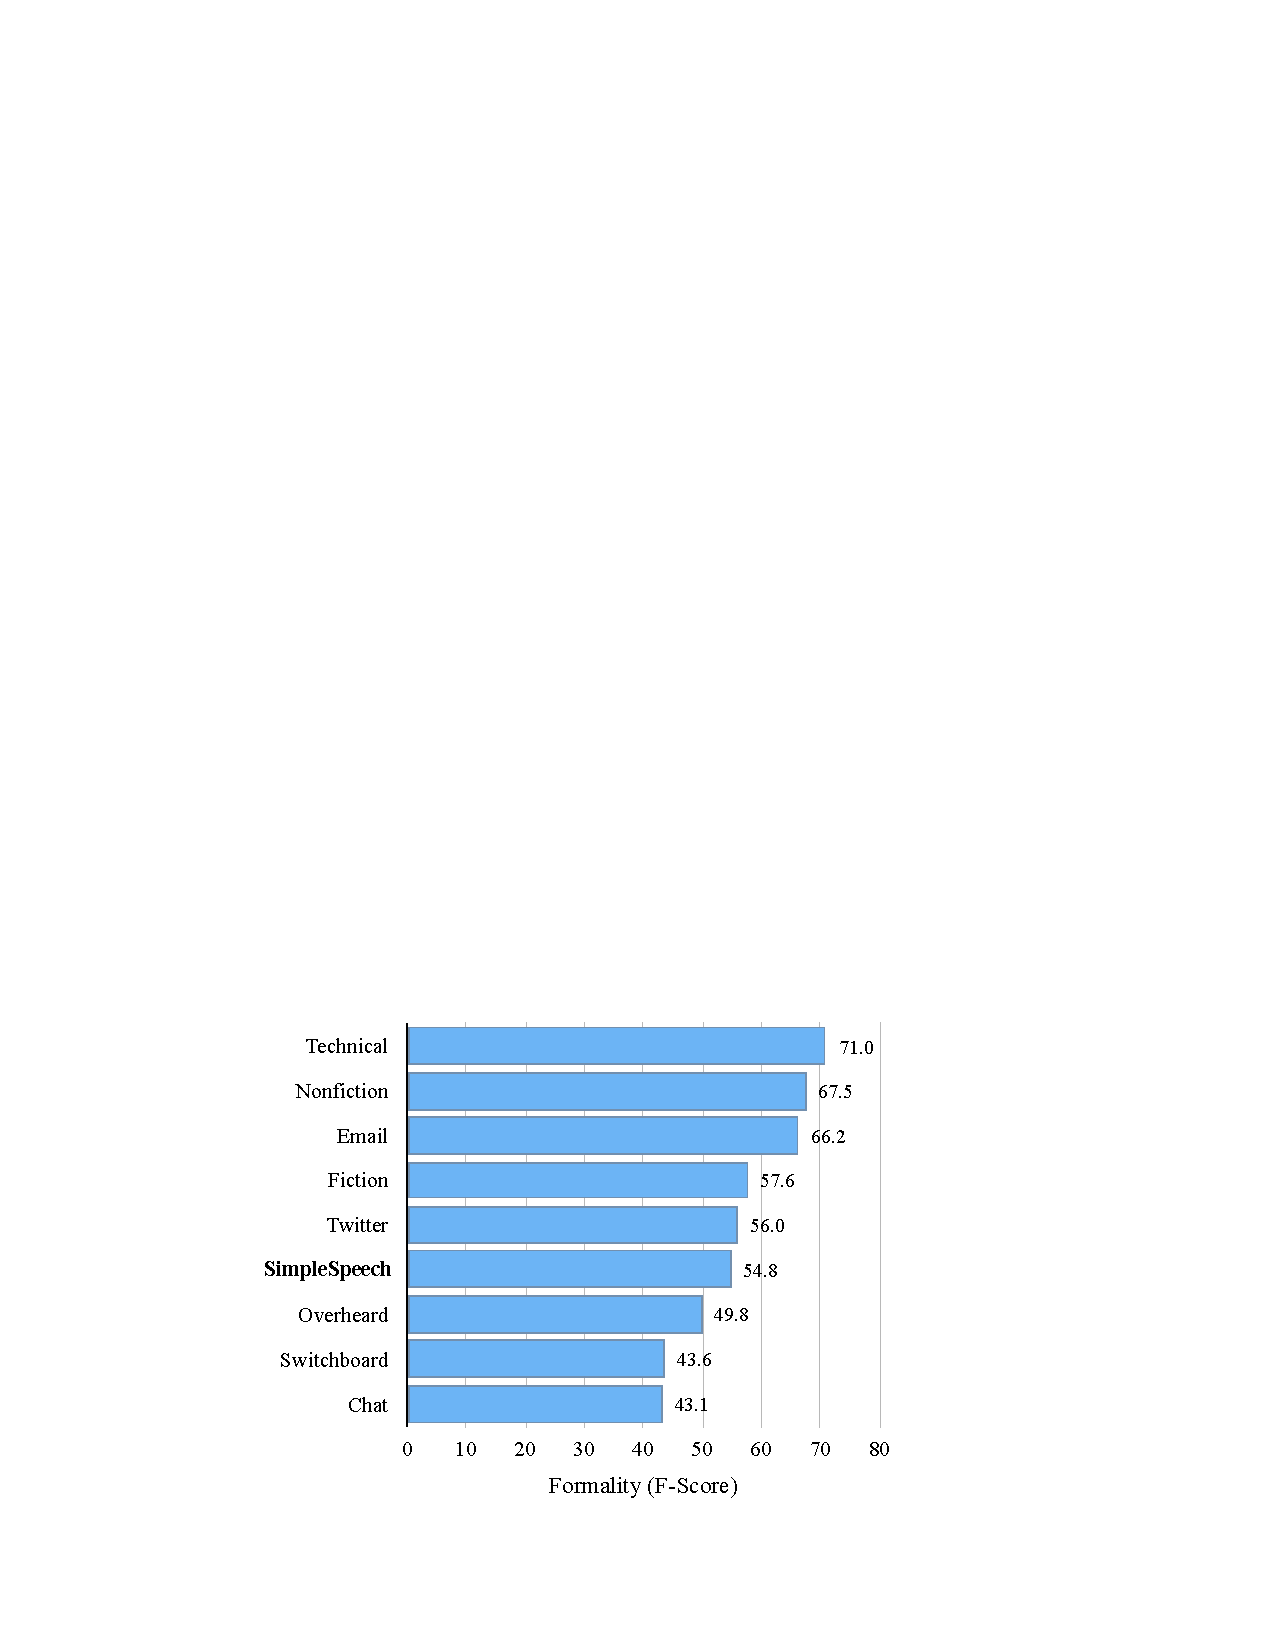
\includegraphics[width=\columnwidth,keepaspectratio]{figures/formality_comparison}
	\caption{The formality of corpora in different genre and media. The messages produced using SimpleSpeech during the quantitative study are intended to reflect general AAC discussion characteristics, and seem to be more formal than other spoken forms of communication but not as formal as email.}~\label{fig:formality}
\end{figure}

\emph{Speaker-audience relationship}. 
Since the F-score is inversely related to contextuality, it is reasonable that the chat and telephone corpora had the lowest F-scores because the participants knew each other and were conversing on a one-to-one basis. 
On the other hand, the written forms of communication (with the exception of email) were more formal because the audience was defined more loosely and not necessarily acquainted with the speaker.
AAC using SimpleSpeech was more closely related to the latter condition (as an online forum discussion), which probably contributed to its greater formality compared to the other spoken corpora.

\emph{Immediacy of communication}. 
The tendency to speak or write more contextually when the recipient replies immediately explains why the online chat text, though written, was more contextual and less formal than the oral corpora. 
It also justifies the fact that the email corpus was more formal than all of the other direct communication media.
Again, AAC falls toward the more formal end of this spectrum because there is little temporal proximity between the speaker and the audience.

\emph{Tendency toward verbosity}.
Media that pressured the creator to be brief or precise were more formal and less contextual.
For instance, writing technical documents requires the preferential use of nouns over pronouns to maximize clarity.
Twitter messages are, of course, limited to 140 characters, leading to a greater concentration of meaning that favors less contextual words.
For AAC, therefore, the ability to edit could influence the contextuality if discussion members were pressured to trim down their recordings. 
For our study, however, the participants were not affected by verbosity; though non-edited recordings had on average 10\% more words than edited ones, these edits were more concentrated on removing disfluencies than improving concision.